\section{UI-Elemente}
\subsection{Buttons}
\begin{itemize}
	\item \textbf{Primär:} Z.B.\ „Anmelden“, „Speichern“, „Weiter“, „Abbrechen“, „Fertig“.
	\item \textbf{Sekundär:} Z.B.\ „Zurück“, „Erneut erinnern“, „Kommentar speichern“.
	\item \textbf{CTA (Call-to-Action):} Z.B.\ „Notfallkontakt anrufen“, „Medikamentenplan öffnen“.
\end{itemize}

Primäre Buttons sind Blau ausgefüllt (\texttt{\#45B3CB}). Sekundäre Buttons sind nicht ausgefüllt, besitzen jedoch einen blauen Rand (\texttt{\#45B3CB}). Dies signalisiert dem Menschen welcher Button für den weiteren Prozess am wichtigsten ist. Sekundäre Buttons zeigen an, dass hier weitere Funktion und zusätzliche Informationen verfügbar sind.

\subsection{Input-Felder}
\begin{itemize}
	\item Textfelder für Telefonnummern, Codes, Geburtsdaten, Symptombeschreibungen.
	\item Datepicker für Zeit und Datum.
	\item Kommentartextfelder (max. 1000 Zeichen).
\end{itemize}

\subsection{Dropdowns \& Listen}
\begin{itemize}
	\item Dropdowns für Datumsauswahl, Messrhythmus (z.B. täglich, wöchentlich).
	\item Listen für Kontakte, Erinnerungen, Messwerte, Medikation.
\end{itemize}

\begin{figure}[!h]
	\centering
	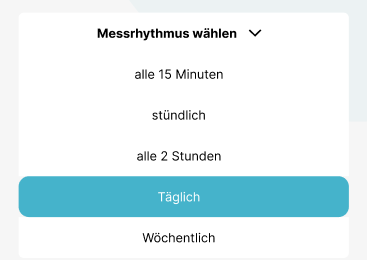
\includegraphics[width=0.45\linewidth]{images/Dropdown}
	\caption{Dropdown-Menü für den Messrhythmus bei Blutdruck \& Puls}
	\label{fig:dropdown}
\end{figure}

\subsection{Navigation}
\begin{itemize}
	\item Hauptmenü mit Modulen wie Erinnerungen, Kontakte, Blutdruck \& Puls, Datenexport, Symptomtagebuch.
	\item Onboarding-Seiten für Registrierung, Einführung, Konfiguration.
\end{itemize}

\subsection{States (Normal, Hover, Disabled, Active)}
\begin{itemize}
	\item \textbf{Normal:} Standardzustand bei Buttons, Eingabefeldern.
	\item \textbf{Disabled:} Buttons ausgegraut, wenn Eingaben fehlen oder Funktion nicht verfügbar ist.
	\item \textbf{Active:} Aktiver Menüpunkt oder laufende Messung (z.\,B.\ Fortschrittsanzeige „30\,\%“).
\end{itemize}

\newpage
